\graphicspath{{chapters/images/07/}}
\chapter{16S-rRNA sequencing}

\section{Introduction to metagenomics}

  \subsection{Definition of metagenomics}
    The term \textbf{metagenomics} refers to the "\textit{study of \textbf{uncultured microorganisms} from the environment, which can include humans or other living hosts}" whith "\textit{focus on taxonomic and functional characteristics of the \textbf{total collection of microorganisms} within a community}". The main way to analyze the entire microbial population of an environment is through \textbf{high-throughput sequencing} of nucleic acids isolated from the sample; we can further distinguish two approaches, namely \textbf{16S rRNA gene sequencing} and \textbf{shotgun  metagenomics}.

  \subsection{Why studying the metagenome}
    Microbes are basically everywhere, in and outside of our bodies, in oceans, glaciers, hot springs and rocks. Given how widespread and abundant microbes are, studying the metagenome provides us plenty of information (both on human and non-human microbiome and environment). For instance, it has been shown that the microbiome correlates to several diseases, therefore it can be used as a non-invasive \textbf{biomarker} (colorectal cancer, immunotherapy efficacy, autoimmune diseases...); the list of activities microbes are involved in is evergrowing.

  \subsection{Differences with older microbiome studies}
    The microbiome was discovered many years ago but there were no tools to analyze it properly; the only way was to culture and isolate each bacterium, which is an unfeasible approach to study the entire community, since only some bacteria can be grown in lab and it still would take an unreasonably long amount of time. The advent of high-throughput technologies is what made possible to study the microbiome of a sample, reducing significantly times, costs and increasing substantially the fraction of the microbiome that can be known.

  \subsection{Example: skin microbiome}
    Some studies were performed on skin microbiome (Segata et al, Nature Methods 2012, Truong et al, Nature Methods, 2015); only about 60\% of the contigs (of various size) were mapped to known microbes while 40\% belonged to unknown species. When separating these sequences based on GC content and abundance, many clusters formed, some with higher abundance while others with lower abundance, probably due to the low GC content that makes more difficult for the machine to sequence them, therefore causing them to be underestimated. Studying this 40\% of unknown sequences is one of the main tasks of metagenomics.

\section{16S rRNA sequencing}

  16S rRNA sequencing is one of the first techniques developed to study the microbiome, since it does not require a huge amount of sequences nor excessive costs; for these reason the technique became popular.

  \subsection{Simplified 16S rRNA analysis workflow}
    The general workflow for a 16S rRNA analysis is the following:
    \begin{itemize}
      \item \textbf{DNA extraction} from the entire community present in the sample; some bacteria will be over-represented while other will be under-represented.
      \item \textbf{Selective PCR amplification of 16S rRNA gene} (due to the characteristics explained below)
      \item \textbf{High-throughput sequencing}
      \item \textbf{Sequence mapping} against genomes in databases; this allows to define which bacteria (and which variants of those) are present in the sample and to find new and unknown bacteria.
    \end{itemize}

    \begin{figure}[!h]
      \centering
      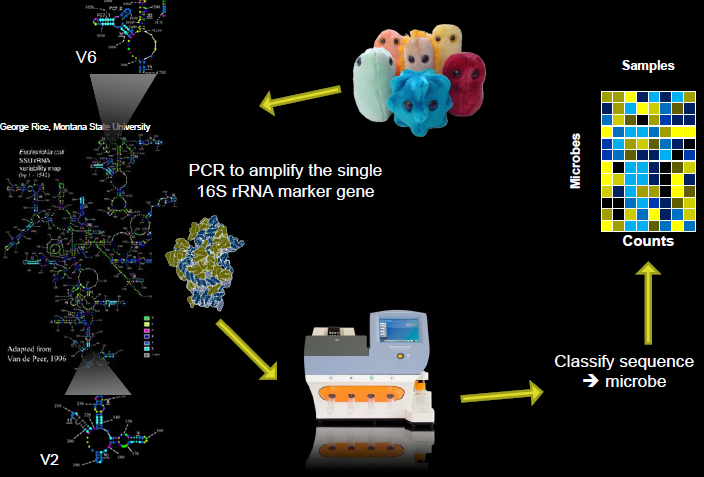
\includegraphics[width=0.9\textwidth]{general_workflow.png}
      \caption{\label{fig:general_workflow}General 16S gene analysis workflow}
    \end{figure}

  \subsection{16S rRNA gene}
    The ribosome is one of the most conserved, if not the most conserved, structure in all living organisms, making it one of the best phylogenetic markers. In prokaryotes, the ribosome is composed of several elements, both proteic and RNA based. Of the RNA based ones, 3 of them are \textbf{ribosomial RNAs} (rRNAs), namely 5S, 16S, 23S. Since these components are fundamental for any bacterium, all bacteria present the genes codifying for these rRNAs; most of the sequences are highly conserved but some regions have some variability which, since this variability is species-specific, can be used as a \textit{barcode} to find and classify species (it also allows to distinguish between Archea and Bacteria).
    The most conserved of the rRNAs is 23S but the one used for microbiome analysis is 16S (which corresponds to the human 18S). The 16S rRNA gene is a few thousands nucleotides long, most of which are highly conserved; the bulk of the differences among species is in the hypervariable regions (named V1 to V9), which are terminal loops of the structure (basically regions far away from the catalityc site, therefore more free to mutate). Despite the high degree of conservation, some variability can be found outside the hypervariable regions too (eg. 530 loop structure).
    The annotation of which portions of the 16S rRNA gene are conserved has been performed using \textit{E. coli} as a reference; for a few hundred organisms the gene has been compared to the reference one to define the degree of conservation of each stretch of nucleotides. Some totally conserved regions (meaning pretty much identical in all species) are present but they are not very big.

    \begin{figure}[!h]
      \centering
      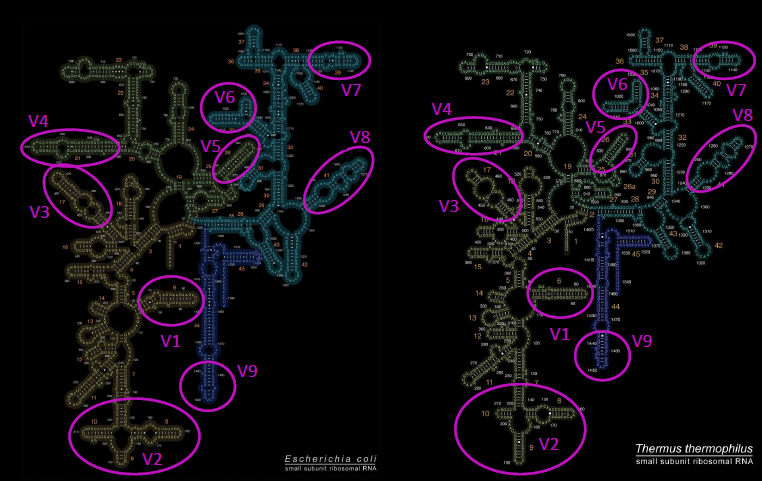
\includegraphics[width=0.9\textwidth]{16S_rRNA.png}
      \caption{\label{fig:16S_rRNA}Structure of the 16S rRNA in \textit{E. coli} and \textit{T. termophilus}}
    \end{figure}

  \subsection{Primer and high-throughput machine choice}
    One could sequence the entirety of the 16S rRNA gene, for example using NanoPore seq, but this would introduce many errors that could lead to mapping the sequence to the wrong organism; for this reason it is preferred to amplify only certain specific regions of the gene.
    To study the microbiome in a high-thoughput way you need primers which can bind to all species, but since the sequences conserved in all species are too short, you use primers that bind highly conserved regions; for this reason, regardless of which primers you choose there will be bias in your results (some species will not be identifiable using those primers). This bias can be somewhat minimized using \textit{in silico} primer validation, which means testing your primers against databases of 16S tRNA genes (silva and green genes), to test and decide the best pair of primers for your experiment.

    \begin{figure}[!h]
      \centering
      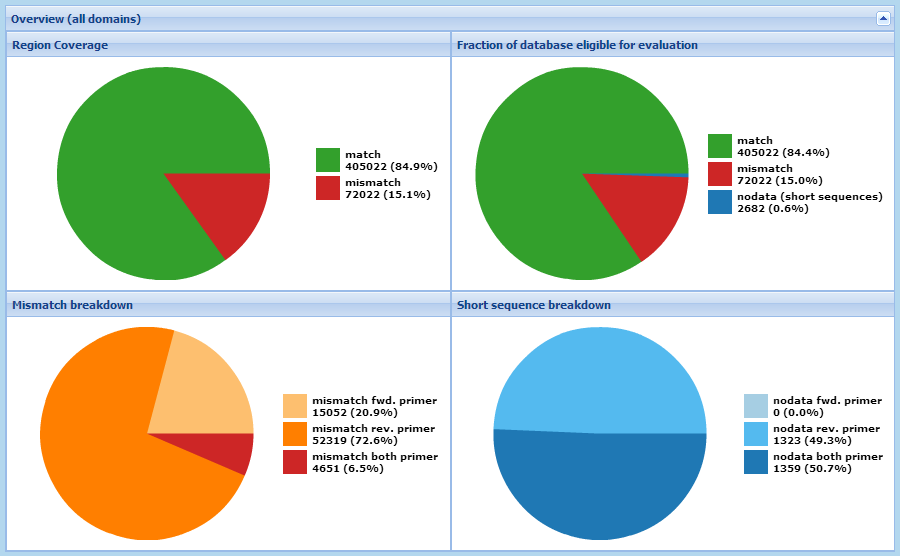
\includegraphics[width=0.9\textwidth]{silva_analysis.png}
      \caption{\label{fig:silva_analysis}Example of \textit{in silico} primer validation using silva; you can notice the different efficiency of the primers relative to different parameters.}
    \end{figure}

    Still, two experiments conducted with different primers will always have some differences.
    Moreover the binding regions must flank some variable region, in order to include it in the amplicon; finally you need pair end amplification (both primer back and forward) in order to have the complete amplicon (to make comparison easier). Given these characteristics there are multiple possible priming sites, based on the sequence and on chemical properties of the primers. Moreover, primers can be used as forward or reverse to obtain different combinations and sequences.

    \begin{figure}[!h]
      \centering
      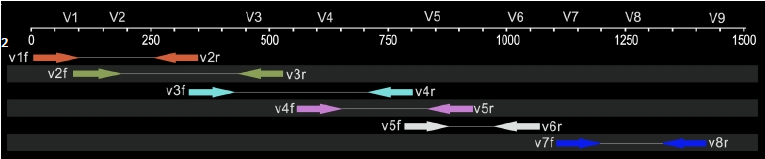
\includegraphics[width=0.9\textwidth]{primer_placement.png}
      \caption{\label{fig:primer_placement}Examples of common primer placements relative to hypervariable regions}
    \end{figure}

    As an example of the importance of the choice of primers, in some skin microbiome analyses, researchers could not find two bacteria always present on human skin due to the choice of primers. Moreover \textit{S. aureus} seemed over-represented due to the non-amplification of other important species. Despite the biases, this technique is still extremely useful even today.

    There are different protocols to target conserved regions also based on the machine used. In general:
    \begin{itemize}
      \item Sanger machines are not very good for this application since they have low throughput and they are more suited for longer sequencing tasks (full genomes for instance)
      \item Roche 454 machines have historically been well suited, since it was possible to sequence three hypervariable regions toghether using 400 nucleotides reads, providing a good cost/throughput trade-off.
      \item Illumina HiSeq is not the optimal choice since it has shorter reads and unnecessarely high througput; Illumina MiSeq and IonTorrent can be a decent compromise.
    \end{itemize}

  \subsection{In depth 16S rRNA analysis workflow}
    A more in depth 16S rRNA analysis worflow is the following:
    \begin{itemize}
      \item \textbf{DNA extraction} from each of your samples
      \item \textbf{Selective PCR amplification of 16S rRNA gene}, introducing a barcode in the sequences using tagged primers.
      \item \textbf{High-throughput sequencing} of all the samples in a single run (to reduce costs); the result is a set of amplicons belonging to different samples and with a barcode attached.
      \item \textbf{Demultiplexing}, which means removing the barcodes and assigning each sequence  to the corresponding sample. Sequencing noise must be taken into account, therefore low quality reads must be removed.
      \item \textbf{Multiple sequence alignment} against reference sequences. Some reads will probably not map to any reference sequence.
      \item \textbf{Group related sequences into OTUs} (operational taxonomic units), which means grouping sequences that share some common variants; since there are some SNPs in the microbial genome, the similarity threshold between sequences cannot be too restrictive. OTUs can be used to define the relative abundance of each species in the sample, but in order to do so it is necessary to normalize for the copy number of the 16S gene sequence; this is very difficult since an accurate estimate can be made only if long reach sequencing has been performed on the organism, which is almost never the case since for microbes that basically corresponds for full genome mapping (needless to say it is therefore non applicable on unknown microbes).
      \item \textbf{Build phylogenetic tree} using one representative for each OTU.
      \item \textbf{Annotate} the OTUs using 16S gene databases.
      \item \textbf{Downstream analysis} is performed, such as clustering to visualize similarities among samples.
    \end{itemize}

    \begin{figure}[!h]
      \centering
      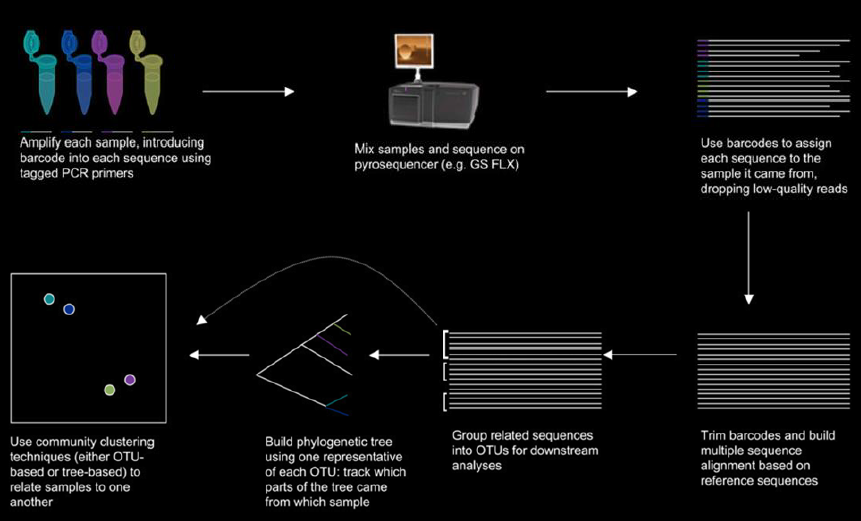
\includegraphics[width=0.9\textwidth]{expanded_workflow.png}
      \caption{\label{fig:expanded_workflow}Expanded 16S gene analysis workflow}
    \end{figure}

    \begin{figure}[!h]
      \centering
      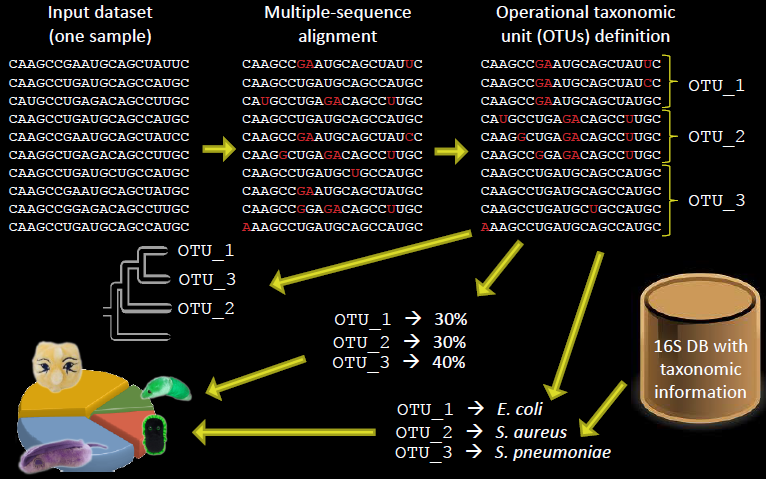
\includegraphics[width=0.9\textwidth]{zoom_in_16S.png}
      \caption{\label{fig:zoom_in_16S}Zoom in on 16S gene analysis workflow}
    \end{figure}

  \subsection{OTU clustering}
    Defining OTUs requires using multiple sequence alignment; since this approach is a generalization of the mapping algorithm (meaning you have to compare every sequence with every sequence) it is quite complex in terms of speed, but still feasible. Generally, greedy algorithms, which add the lowest possible amount of gaps, are used to perform multiple sequence alignment. After the alignment, sequences are split into OTUs (operational taxonomic units), which are basically groups of 16S sequences very similar to each other. Generally a sequence is defined as the representative of the OTU, meaning that it has a certain threshold of identity with all other sequences in the OTU (usually 97\% when considering species) and that minimizes the differences of all other sequences of the OTU with itself. Some OTUs can be assigned univocally to a species, some others may be associated to more species, some others cannot be mapped to know species. The fact that a species may map to multiple OTUs is often a negative factor (confusion in the analysis) but it may sometimes allow to find subspecies.
    \begin{figure}[!h]
      \centering
      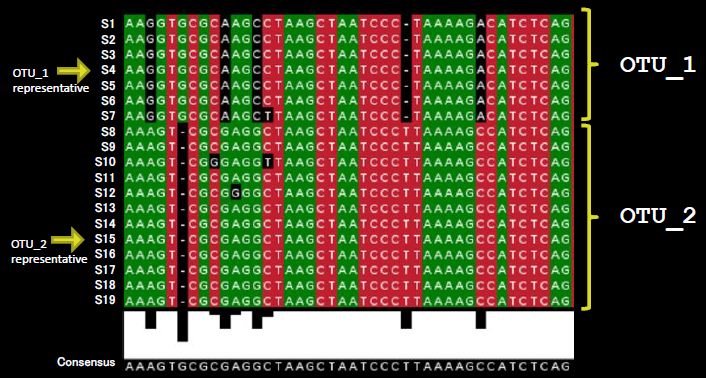
\includegraphics[width=0.9\textwidth]{OTU_general.png}
      \caption{\label{fig:OTU_general}Example of multiple sequence alignment for OTUs}
    \end{figure}

    After sequence alignment, OTU clustering (= splitting the sequences into OTUs), can be done through several supervised or unsupervised learning methods. Each methods has pros and cons, therefore there is not an always optimal method.
    The most common unsupervised clustering methods are:
    \begin{itemize}
      \item \textbf{Single linkage clustering} (nearest neighbour): assign the sequence to a cluster if that OTU already contains \textbf{at least a sequence} similar enough (97\%). However two distant sequences in the OTU network could share a similarity which is way lower than 97\% (because of a series of connections above 97\%); this could result in \textbf{underclustering} (defining too few clusters).
      \item \textbf{Complete linkage clustering} (furthest neighbour): assign the sequence to a cluster only if \textbf{all the sequences} of the OTU are similar enough (97\%). However two sequences may be similar enough (97\%), yet belong to different OTUs, because the overall cluster width, or \textbf{divergence}, is at most 3\%; this approach could then generate different solutions, based on the order the points are added in. Moreover, if the clustering conditions are too stringent, sequencing errors and SNPs in the microbial genome may result in \textbf{overclustering} (defining too many clusters).
    \end{itemize}

    \begin{figure}[!h]
      \centering
      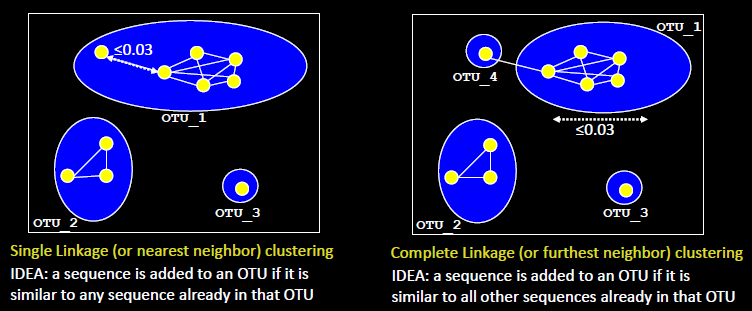
\includegraphics[width=0.9\textwidth]{clustering_methods.png}
      \caption{\label{fig:clustering_methods}Visualization of single linkage analysis and complete linkage analysis}
    \end{figure}

    \begin{figure}[!h]
      \centering
      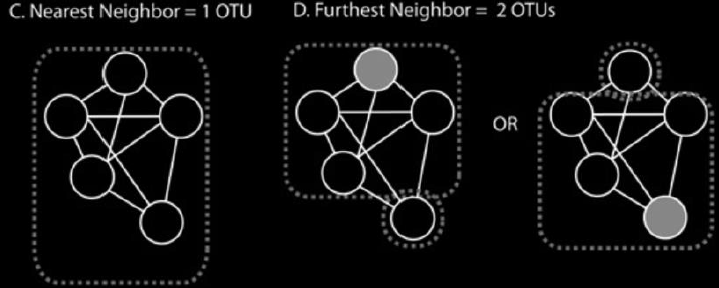
\includegraphics[width=0.9\textwidth]{overclustering.png}
      \caption{\label{fig:overclustering}Example of overclustering and result multiplicity due to complete linkage analysis}
    \end{figure}

  \subsection{OTU taxonomic annotation}
    \textbf{NOTE: this topic continues in the next lecture; when done merge together}
    Assigning a taxonomic annotation to an OTU cannot be done simply using BLAST to get the best matching sequence; this is because there is too much noise in the sequences and because it is difficult to classify new strains. A better way is using some other algorithm that assigns the terms of the taxonomic notation (since it is more than just one label) and provides some degree of confidence in the prediction. For instance the algorithm may be able to correctly assign the first taxonomical terms, up until \textit{Enterobacteriaceae}, but then it provides a prediction of the OTU belonging to \textit{E. coli} with some confidence interval, say 85\%, and some alternative like \textit{S. dysenteriae}, say with 15\% confidence.
